% !TeX spellcheck = en_GB
\documentclass[12pt,fleqn]{article}

\usepackage[english]{babel}
\usepackage{SpeedyGonzales}
\usepackage{MediocreMike}
%\usepackage{Blastoise}

\title{}
\author{Asger Schultz}
\date{\today}

\fancypagestyle{plain}
{
	\fancyhf{}
	\rfoot{Side \thepage{} af \pageref{LastPage}}
	\renewcommand{\headrulewidth}{0pt}
}
\pagestyle{fancy}
\fancyhf{}
\lhead{Asger Schultz}
\chead{}
\rhead{}
\rfoot{Side \thepage{} af \pageref{LastPage}}

\graphicspath{{Billeder/}}
\linespread{1.15}


%\numberwithin{equation}{section}
%\numberwithin{footnote}{section}
%\numberwithin{figure}{section}
%\numberwithin{table}{section}

\begin{document}

\maketitle
%\thispagestyle{fancy}
%\tableofcontents
-- Compare measurement methods of bioavailable phosphorous and examine the influence of bioavailable phosphorous on harvest yield. 
-- By the explanatory strengths of the two measurements, the DGT measurement is found to be most useful in predicting the yield.
-- Bioavailable phosphorous is using both measurements found to have significant effect on the yield \(p<10^{-9}\).
\tableofcontents
\newpage 
\section{Introduction}
A wide range of very different effects are in play in determining the output yield of a farm.
As environmental and economic incentives rise, there is increasing motivation for precision agriculture which optimizes the performance of farming using ecological, chemical and biological variables.
One of these important variables is the nutrient of the soil and \textit{phosphorous} is essential in this regard.


This report considers different techniques for measuring the amount of phosphorous available to the plants and compares two measurement methods, the traditional "Olsen-P" and the newer "DGT" method, using the output yield of barley fields as the target.  
Correlations, model fitting of Michaelis-Menten models and ANCOVA models are used to examine the connections between the measurements and the yield output.
\section{Data}
The data consists of 100 observations each consisting continuous  Olsen-P measurements [mg/100g], DGT-measurements [\(\mu\)g/L] and harvest yield of barley [hkg/ha] and categorical location id's for the field on which the observations were made. Nine fields have been surveyed and given id's from "001" to "011". The last field has missing values for two of it's three yield measurements.  

The fields are from Denmark and Norway and the multiple 
\section{Methods and analysis}
\subsection{Recommended measure}
-- Correlation and corr test\\
-- Fit of Michaelis-Menten model\\
-- Consider 
\subsection{Yield influence of bioavailability}
--ANCOVA using DGT and location\\
--ANCOVA using olsenP and location
\section{Results}
\begin{figure}[H]
	\centering
	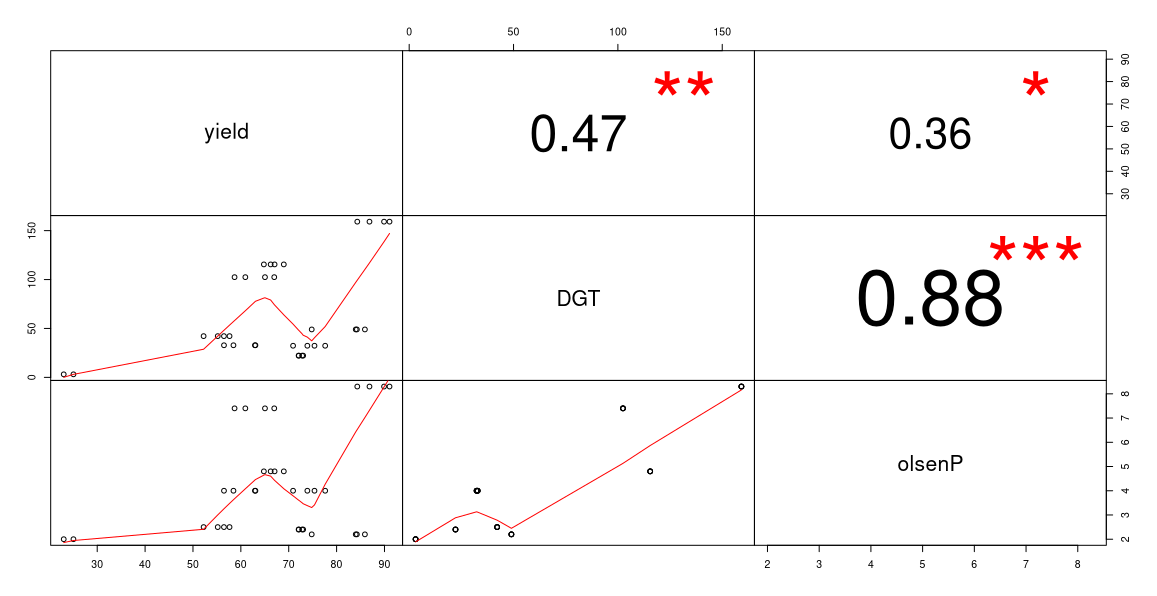
\includegraphics[width=.9\linewidth]{p2_corrplot}
	\caption{Visualization of a Correlation Matrix. On top the (absolute) value of the correlation plus the result of the cor.test as stars. On bottom, the bivariate scatterplots, with a fitted line}
\end{figure}
\begin{figure}[H]
	\centering
	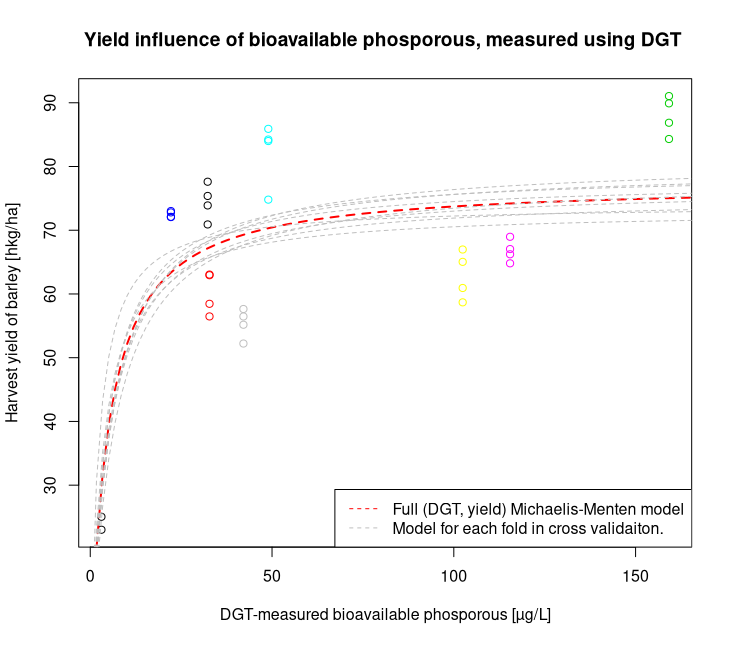
\includegraphics[width=.8\linewidth]{dgt_mmm}
\end{figure}
\begin{figure}[H]
	\centering
	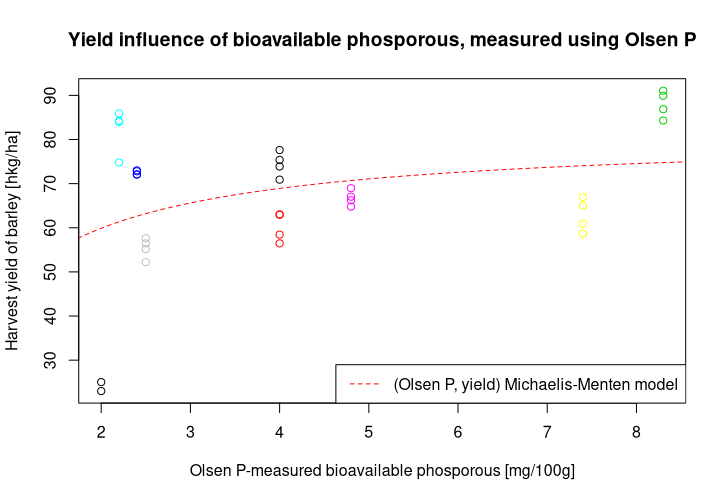
\includegraphics[width=.8\linewidth]{oP_mm}
\end{figure}

\begin{align*}
	& \sqrt{MSE_{dgt}}	 = 10.84
	&& \sqrt{MSE_{olsenP}} = 14.65
\end{align*}
%\begin{figure}[H]
%	\centering
%	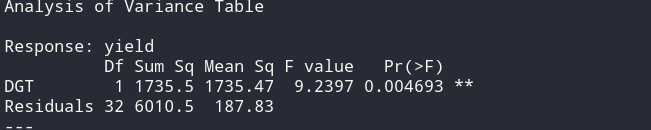
\includegraphics[width=.7\linewidth]{simpleDGT}
%\end{figure}



%\begin{figure}[H]
%	\centering
%	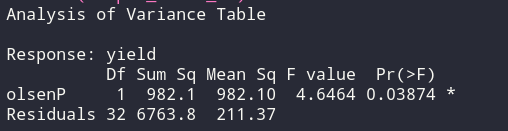
\includegraphics[width=.7\linewidth]{simpleOP}
%\end{figure}
\begin{figure}[H]
	\centering
	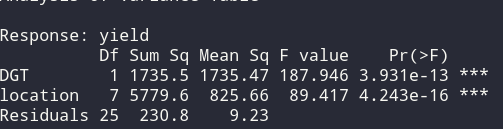
\includegraphics[width=.7\linewidth]{anovaDGT}
\end{figure}
\begin{figure}[H]
	\centering
	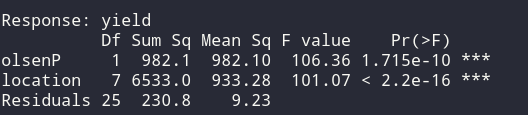
\includegraphics[width=.7\linewidth]{anovaOP}
\end{figure}

\section{Discussion}

\end{document}

















